\begin{frame}
  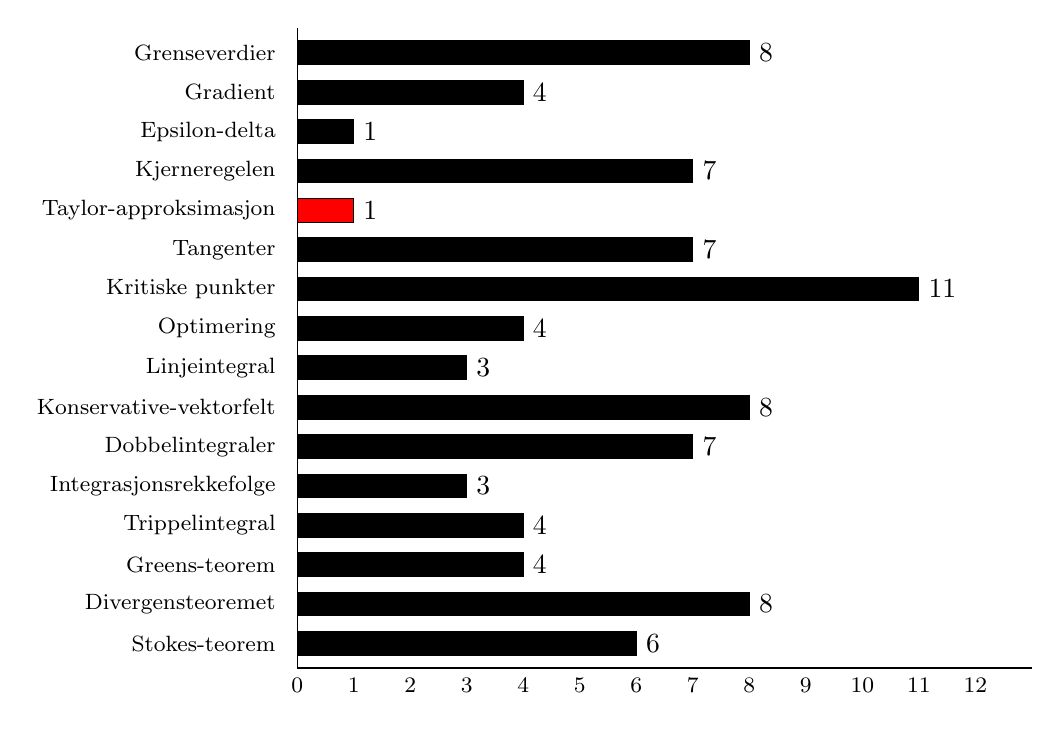
\begin{tikzpicture}
    \begin{axis}[ xbar=0pt, /pgf/bar shift=0pt, legend style={ legend columns=4,
        at={(xticklabel cs:0.5)}, anchor=north, draw=none }, ytick={0,...,15},
      ytick style={draw=none},% <- added
      axis y line*=none, axis x line*=bottom, tick label
      style={font=\footnotesize}, legend style={font=\footnotesize}, label
      style={font=\footnotesize}, xtick style={draw=none},% <- added
      xtick={0,1,...,12}, width=.9\textwidth, bar width=3mm, y dir = reverse,
      xmin=0, xmax=13, area legend,
      y=5mm, enlarge y limits={abs=0.625},
      style={text=black}, every axis plot/.append style={fill},
      nodes near coords, nodes near coords,
      yticklabels={%
        {\topicref{Grenseverdier}},
        {\topicref{Gradient}},
        {\topicref{Epsilon-delta}},
        {\topicref{Kjerneregelen}},
        {\topicref{Taylor-approksimasjon}},
        {\topicref{Tangenter}},
        {\topicref{Kritiske punkter}},
        {\topicref{Optimering}},
        {\topicref{Linjeintegral}},
        {\topicref{Konservative-vektorfelt}},
        {\topicref{Dobbelintegraler}},
        {\topicref{Integrasjonsrekkefolge}},
        {\topicref{Trippelintegral}},
        {\topicref{Greens-teorem}},
        {\topicref{Divergensteoremet}},
        {\topicref{Stokes-teorem}}}]
      \addplot[fill=black] coordinates {(8,0)};
      \addplot[fill=black] coordinates {(4,1)};
      \addplot[fill=black] coordinates {(1,2)};
      \addplot[fill=black] coordinates {(7,3)};
      \addplot[fill=red] coordinates {(1,4)};
      \addplot[fill=black] coordinates {(7,5)};
      \addplot[fill=black] coordinates {(11,6)};
      \addplot[fill=black] coordinates {(4,7)};
      \addplot[fill=black] coordinates {(3,8)};
      \addplot[fill=black] coordinates {(8,9)};
      \addplot[fill=black] coordinates {(7,10)};
      \addplot[fill=black] coordinates {(3,11)};
      \addplot[fill=black] coordinates {(4,12)};
      \addplot[fill=black] coordinates {(4,13)};
      \addplot[fill=black] coordinates {(8,14)};
      \addplot[fill=black] coordinates {(6,15)};
    \end{axis}
  \end{tikzpicture}
\end{frame}

\begin{frame}
  \subsection{Taylor-approksimasjon}\label{subsec:Taylor-approksimasjon}
  \frametitle{Taylor-approksimasjon}
  Some more text here
\end{frame}

\begin{frame}
  \begin{oppgave}{K2016, Oppgave 3}
    La $f(x,y) = x^4 + x^3 + y^2 + xy$. Finn andreordens Taylor-approksimasjon
    av $f$ i $(x_0, y_0) = (1,2)$.
  \end{oppgave} \visible<2->{\textbf{Steg 1:} Regn ut de partiellderiverte
  \begin{align*}
    & f_x(x,y) = 4x^3 + 3x^2 + y
      && \Rightarrow && f_x(1,2) = 9 \\
    & f_{xx}(x,y) = 12x^2 + 6x
      && \Rightarrow && f_{xx}(1,2) = 18 \\
    & f_{y}(x,y) = 2y + x
      && \Rightarrow && f_{y}(1,2) = 5 \\
    & f_{yy}(x, y) = 2
      && \Rightarrow && f_{yy}(1,2) = 2 \\
    & f_{xy}(x,y) = 1
      && \Rightarrow && f_{xy}(x,y) = 1 \\
    & f_{yx}(x,y) = 1
      && \Rightarrow && f_{yx}(x,y) = 1 \\
  \end{align*}}
\end{frame}

\begin{frame}
  \begin{oppgave}{K2016, Oppgave 3}
    La $f(x,y) = x^4 + x^3 + y^2 + xy$. Finn andreordens Taylor-approksimasjon
    av $f$ i $(x_0, y_0) = (1,2)$.
  \end{oppgave}
  \textbf{Steg 2:} Sett inn $\X^0 = (x_1^0,x_2^0)=(1,2)$ og $\X =
    (x_1, x_0) = (x,y)$ i formel.
    \begin{align*}
      T_2(\X) & = 
    \only<1-2>{f(\X^0)
               + \sum_{i=1}^{n} \only<1>{\diffp{f}{{x_i}}}%
                              \only<2>{f_{x_i}}(\X^0)(x_i - x_i^0)%
               + \frac{1}{2} \sum_{i,j=1}^{n} \only<1>{\diffp{f}{{x_i}{x_j}}}%
                                            \only<2>{f_{{x_i}{x_j}}}(\X^0)(x_i-x_i^0)(x_j - x_j^0)} 
    \only<3->{\underbrace{f(\X^0)}_{(1)}
      + \underbrace{\sum_{i=1}^{n} f_{{x_i}} (\X^0)(x_i - x_i^0)}_{(2)}
      + \underbrace{\frac{1}{2} \sum_{i,j=1}^{n} f_{{x_i}{x_j}}(\X^0)(x_i-x_i^0)(x_j - x_j^0)}_{(3)}} \\
    \only<5-14>{& = (8)} \only<10-14>{+ (9x + 5y - 19)} \only<14>{+ (9 x^2 + x y - 20 x + y^2 - 5 y + 15)}
    \only<15->{& = 4 - 11x + 9 x^2 + y^2 + xy }
  \end{align*}
  \begin{align*}
    \only<4-5>{(1)
    \mid f(\X^0) =} \only<4>{f(1,2)} \only<5>{8}
      \only<6-10>{(2)
    \left|\,\only<6>{\sum_{i=1}^{n} f_{{x_i}} (\X^0)(x_i - x_i^0)}
         \only<7->{\sum_{i=1}^{2} f_{{x_i}} (1,2)(x_i - x_i^0)} \right.
      \only<8>{= f_x(1,2) \cdot (x-1) + f_y(1,2) \cdot (y-2)} 
      \only<9>{= 9 (x-1) + 5(y-2)}
      \only<10>{= 9x + 5y - 19}}
    \only<11-14>{(3)
    & \left|\,
      \frac{1}{2}\sum_{i=1}^2 \sum_{j=1}^2 f_{{x_i}{x_j}}(1,2)(x_i - x_i^0) (x_j - x_j^0)\right. \\
      & = \only<11-12>{\frac{1}{2}f_{xx}(1,2)(x-1)^2 + \only<11>{\frac{1}{2}}f_{xy}(1,2)(x-1)(y-2) + \only<11>{\\
    & \hspace{4cm} \frac{1}{2}f_{yx}(1,2)(y-2)(x-1) +} \frac{1}{2}f_{yy}(1,2)(y-2)^2}}
      \only<13>{\frac{18}{2}(x-1) + 1 \cdot (x-1)(y-2) + \frac{2}{2}(y-2)^2}
      \only<14>{9 x^2 + x y - 20 x + y^2 - 5 y + 15}
  \end{align*}
\end{frame}

\begin{frame}
  \begin{oppgave}{K2016, Oppgave 3}
    La $f(x,y) = x^4 + x^3 + y^2 + xy$. Finn andreordens Taylor-approksimasjon
    av $f$ i $(x_0, y_0) = (1,2)$.
  \end{oppgave}
  \includegraphics[width=0.5\textwidth]{../img/taylor-zx}%
  \includegraphics[width=0.5\textwidth]{../img/taylor-zy}
\end{frame}

%%% Local Variables:
%%% mode: latex
%%% TeX-master: "main"
%%% End:
